% To add custom packages to the path, go to: /Users/leonlufkin/Library/texmf/tex/latex
\documentclass{article}
\usepackage{myreport}

\title{Shared Representations Model}
\author{Leon Lufkin}
\date{\today}

\makeatletter
\let\Title\@title
\let\Author\@author
\let\Date\@date

\begin{document}

%%%%%%%%%%%%%%
% Statement %%
%%%%%%%%%%%%%%
\section{Statement}
The goal of this analysis is to understand the shared representations model.

We have words in a dictionary:
\begin{align*}
    \DD \triangleq \{ \bm{x}_1, \ldots, \bm{x}_V \} \subseteq \R^D,
\end{align*}
and a set of $L$ languages, indexed by $[L] = \{ 1, \ldots, L \}$.
For simplicity, we make the following assumption:
\begin{assumption} \label{assumption:one-hot}
    The dictionary $\DD$ is a set of one-hot vectors that span $\R^D$.
    So, $V = D$.
\end{assumption}

We train a gated deep linear network (GDLN) to ``translate'' words from one language into another.
The gated deep linear network is represented by a collection of $L$ input and output weight matrices of dimensions $D \times H$ and $H \times D$, respectively, and a hidden layer of size $H \times H$.
The forward pass of the GDLN is given by:
\begin{align*}
    \hat{y}(\bm{x})
    &= \sum_{l' \in [L]} g_{l'}(\bm{x}) \bm{W}_o^{l'} \bm{W}_h \left( \sum_{l \in [L]} g_l(\bm{x}) \bm{W}_i^l \bm{x} \right) 
    = \sum_{l,l' \in [L]} g_l(\bm{x}) g_{l'}(\bm{x}) \bm{W}_o^{l'} \bm{W}_h \bm{W}_i^l \bm{x}.
\end{align*}
Here, the input $\bm{x}$ contains a one-hot vector for the word we are translating, and an input-output language pair.
To make this more explicit, we will now write inputs as $(\bm{x}, p)$, where $\bm{x}$ is the one-hot word and $p = (k, k')$ is the language pair, where $k,k' \in [L]$ are the languages of the input and output, respectively.
Thus, we write,
\begin{align*}
    \hat{y}(\bm{x}, p)
    &= \underbrace{ \Bigg[ \sum_{l,l' \in [L]} g_l(p) g_{l'}(p) \bm{W}_o^{l'} \bm{W}_h \bm{W}_i^l \Bigg] }_{\triangleq \bm{A}_{p}} \bm{x},
\end{align*}
where $\bm{A}_{p}$ is a matrix of size $V \times V$ that depends only on the input via the language pair $p$.

During training, we will sample input-output pairs $p$ uniformly from a subset of the language pairs, which we denote $T \subseteq [L]^2$.
We will equivalently use $T$ to denote the cardinality of the set $T$, and $\bm{T}$ to denote a binary matrix, where $\bm{T}_{k,k'} = 1$ if $(k,k') \in T$ and $0$ otherwise.
The gates operate on $p$ as follows: $g_l(p) = \mathbbm{1}(l = k)$ and $g_{l'}(p) = \mathbbm{1}(l' = k')$.

We study \emph{\underline{full-batch} gradient flow}.
For simplicity, we will assume that $y(\bm{x}_v, p) \equiv \bm{x}_{\pi_p(v)}$ where $\pi_p$ is a permutation on $[L]$ corresponding to language pair $p$, i.e., the target is another one-hot vector in the dictionary $\DD$\footnote{I believe this is how Andrew set it up.}.
In particular, we assume $\pi_p = \pi_{k'} \circ \pi_k^{-1}$, where $\pi_k$ is a permutation on the input language $k$ and $\pi_{k'}$ is a permutation on the output language $k'$.
Intuitively, this maps each word in the input language to a word to an abstract representation, and then maps that abstract representation to a word in the output language.
Since these are one-hot vectors (by \cref{assumption:one-hot}), we can also write $\bm{x}_{\pi_p(v)} = \bm{\Pi}_p \bm{x}_v = \bm{\Pi}_{k'} \bm{\Pi}_k^\top \bm{x}_v$, where $\bm{\Pi}_k$ is the permutation matrix corresponding to $\pi_k$.

With this structure, we can write the loss function as:
\begin{align*}
    \LL &= \E_{\bm{x} \sim \DD, p \sim T} \left[ \frac{1}{2} \| \hat{y}(\bm{x}, p) - y(\bm{x}, p) \|^2 \right] \\
    &= \frac{1}{2} \E_{\bm{x} \sim \DD, p \sim T} \left[ \left\Vert \bm{A}_p \bm{x} - \bm{\Pi}_p \bm{x} \right\Vert^2 \right] \\
    % &= \frac{1}{2} \E_{p \sim T} \left[ \E_{\bm{x} \sim \DD} \left[ \left\Vert \bm{A}_p \bm{x} - \bm{\Pi} \bm{x} \right\Vert^2 \right] \right] \\
    &= \frac{1}{2} \E_{p \sim T} \left[ \frac{1}{D} \sum_{i\in[D]} \left[ \left\Vert ( \bm{A}_p - \bm{\Pi}_p ) \bm{e}_i \right\Vert^2 \right] \right] \\ % & \text{\cref{assumption:one-hot}} \\
    &= \frac{1}{2D} \E_{p \sim T} \left[ \left\Vert \bm{A}_p - \bm{\Pi}_p \right\Vert_F^2 \right].
\end{align*}

Expanding $\bm{A}_p$ and summing over $p$ gives:
\begin{align*}
    \LL
    &= \frac{1}{2DT} \sum_{(k,k') \in T} \left\Vert \sum_{l,l' \in [L]} g_l(p) g_{l'}(p) \bm{W}_o^{l'} \bm{W}_h \bm{W}_i^l - \bm{\Pi}_{k'} \bm{\Pi}_k^\top \right\Vert_F^2.
\end{align*}
We use block matrix notation to clean this up; define:
\begin{align*}
    \bm{W}_o &= \begin{pmatrix} \bm{W}_o^1 \\ \vdots \\ \bm{W}_o^L \end{pmatrix} \in \R^{L H \times D}, \\
    \bm{W}_i &= \begin{pmatrix} \bm{W}_i^1 \ \hdots \ \bm{W}_i^L \end{pmatrix} \in \R^{D \times L H}, \\
    \bm{\Pi} &= \begin{pmatrix} \bm{\Pi}_1 \\ \vdots \\ \bm{\Pi}_L \end{pmatrix} \in \R^{L D \times D}, \\
\end{align*}
Then, using $\bm{J}_L$ to denote the $L \times L$ matrix of all ones, we can write:
\begin{align*}
    \LL
    &= \frac{1}{2DT} \left\Vert ( \bm{W}_o \bm{W}_h \bm{W}_i - \bm{\Pi} \bm{\Pi}^\top ) \odot ( \bm{T} \otimes \bm{J}_D ) \right\Vert_F^2,
\end{align*}
where $\otimes$ is the Kronecker product and $\odot$ is the Hadamard product.

I believe Andrew said we could make the following, additional, assumption:
\begin{assumption} \label{assumption:identity}
    The permutation matrices $\bm{\Pi}_k$ can all be taken to be the identity matrix, i.e. $\bm{\Pi}_k = \bm{I}_D$ for all $k \in [L]$.
\end{assumption}
Under \cref{assumption:identity}, the loss function simplifies to:
\begin{align}
    \LL
    &= \frac{1}{2DT} \left\Vert ( \bm{W}_o \bm{W}_h \bm{W}_i - \bm{J}_L \otimes \bm{I}_D ) \odot ( \bm{T} \otimes \bm{J}_D ) \right\Vert_F^2.
    \label{eq:loss}
\end{align}
\underline{This is the loss function we simulate below.}
It is worth noting that we would have obtained the same loss function if we had used $\bm{x} \sim \NN(0, \frac{1}{D} I_D)$ instead of one-hot vectors.

%%%%%%%%%%%%%%%%%
%% Simulations %%
%%%%%%%%%%%%%%%%%
\section{Simulations}
\FloatBarrier
To validate and gain insight our model, we simulate the loss function in \cref{eq:loss}.
We sample $\bm{T}$ by fixing the diagonal to be $1$ and randomly making off-diagonal entries $1$ until we achieve a desired fraction of $1$s; all other entries are set to $0$\footnote{I don't see any inherent reason to make the diagonal all 1s; this is something I would change, but I had sunk too much compute into these sims by the time I realized this.}.
We use JAX to run these experiments, giving us much greater control over randomness and intialization.
In particular, for each seed, when increasing the number of $1$s by one over a previous experiment, we do not resample the entire matrix $\bm{T}$, but rather we only sample one new entry.
Additionally, when change the initialization scale $\sigma$, we do not resample the entire matrix $\bm{W}_o \bm{W}_h \bm{W}_i$, but rather we only rescale the entries of those matrices.

\Cref{fig:loss} shows the results of our simulations.
We see that generalization typically emerges after roughly 30\% of the pairs have been trained on.
However, this is not always the case, and we do see spikes in test loss for some experiments after this point (my initial guess is that this is numerical, but I could also believe that these simulations are highly sensitive to the structure of $\bm{T}$, though I believe Andrew said he did not see this).
Additionally, the generalization threshold appears to \emph{decrease} as the initialization scale $\sigma$ decreases, which suggests that, as $\sigma \to 0$, the generalization threshold may go to zero as well, a counterintuitive result.
Morever, we see considerable variation across random seeds.

\begin{figure}[!ht]
    \centering
    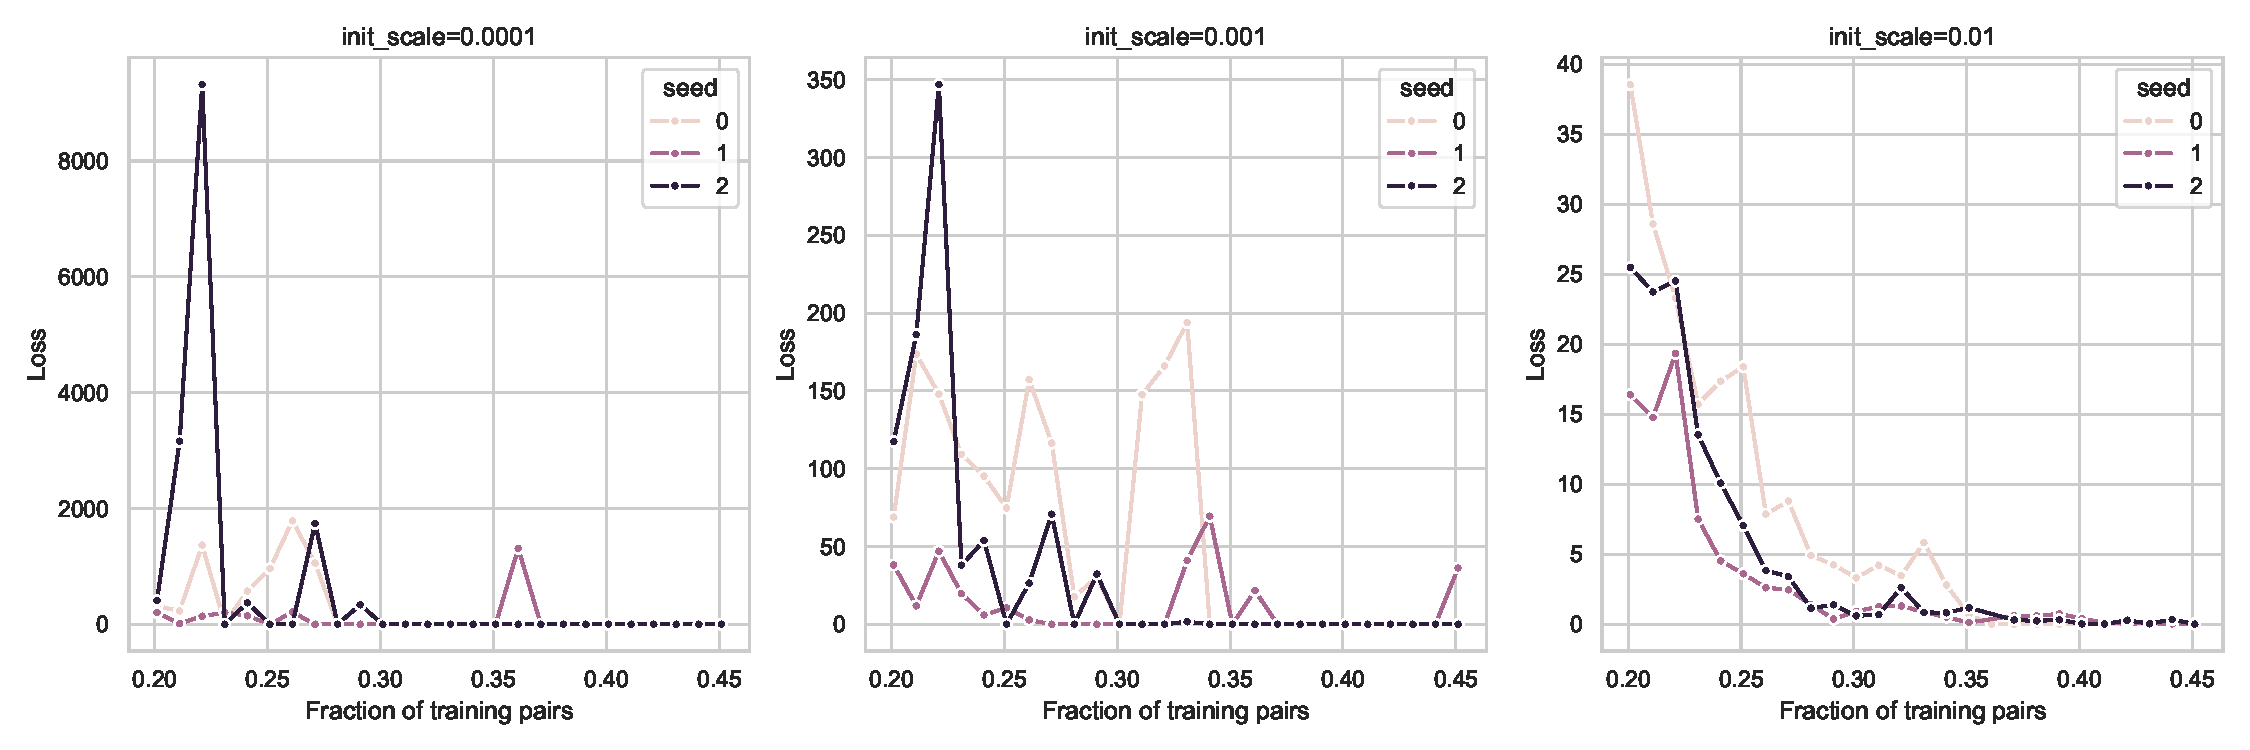
\includegraphics[width=0.8\textwidth]{results_exact.pdf}

    \vspace{1em}

    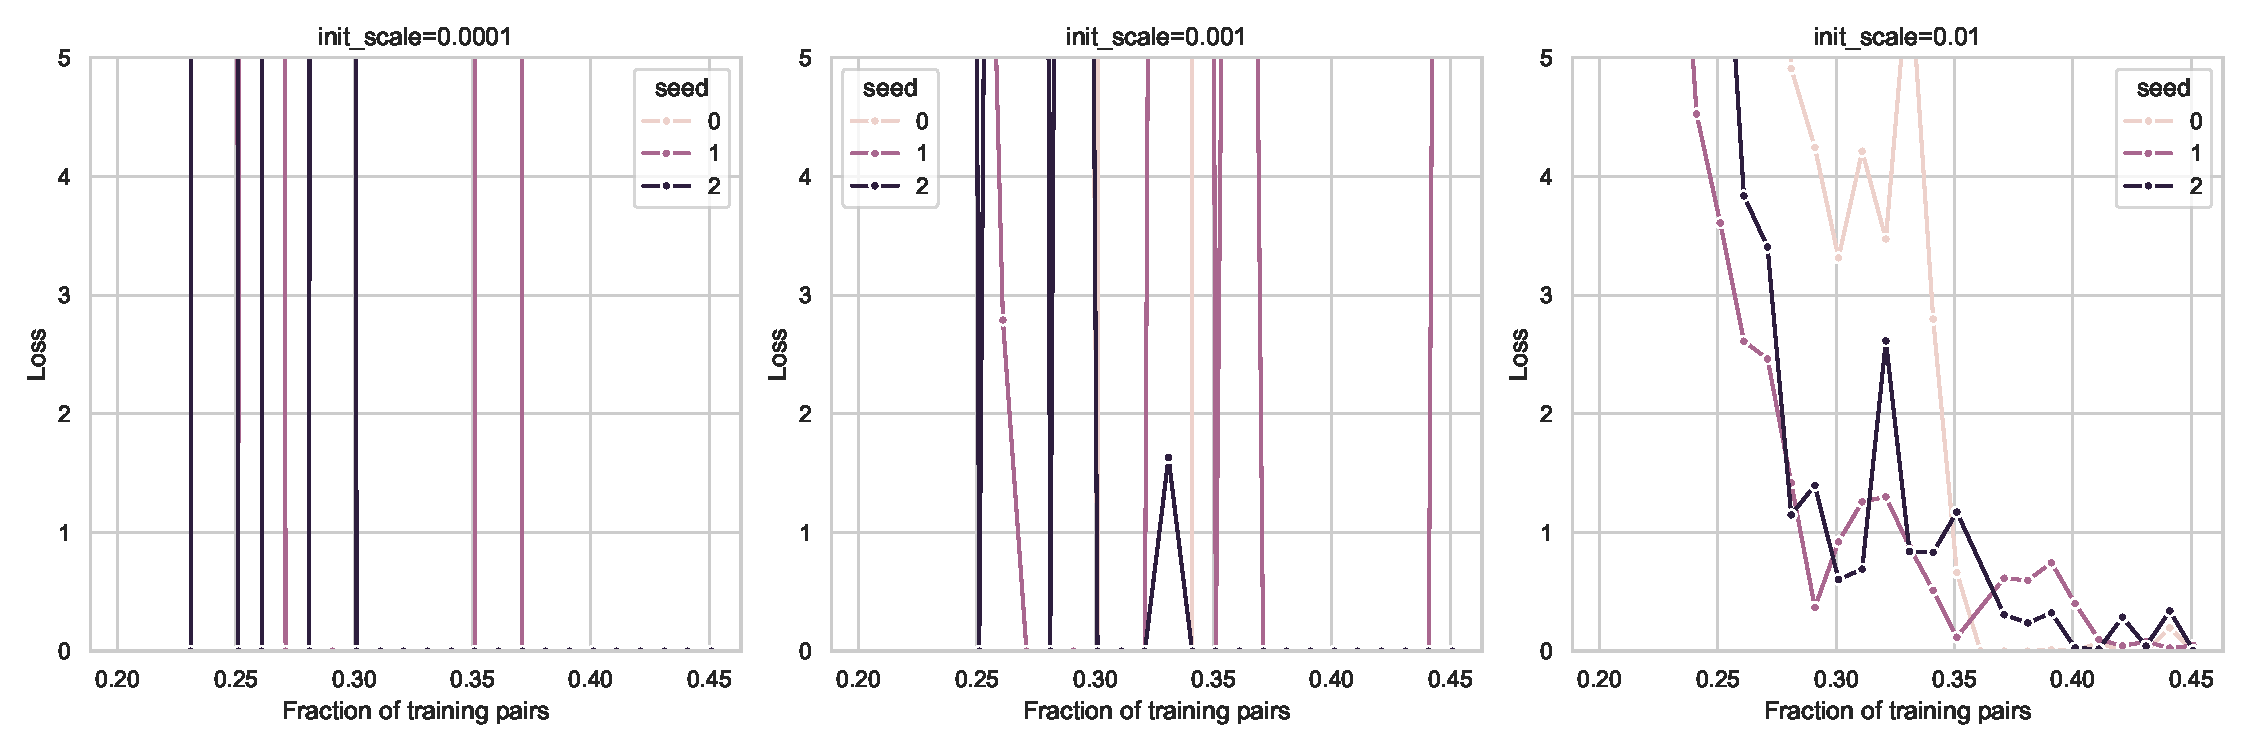
\includegraphics[width=0.8\textwidth]{results_exact_truncated.pdf}

    \caption{(a) MSE loss on \emph{untrained} language pairs after gradient flow achieving a value of $10^{-6}$ on the loss $\LL$ from \cref{eq:loss} for various $\sigma$ and three random seeds.
    (b) Same setup as in (a), but the loss is truncated at $\LL = 5$ to show spikes later in training.
    %
    The model is a GDLN with $L = 10$, $H = 32$, and $D = 32$. Each point represents a single training run.}
    \label{fig:loss}
\end{figure}
\FloatBarrier


%%%%%%%%%%%%%%%%%%%
%% A Simple Case %%
%%%%%%%%%%%%%%%%%%%
\section{A Simple Case}
The block structure of the loss suggests we may be able to gain insight from studying a simpler, non-block, analogue:
\begin{align}
    \LL
    &= \frac{1}{2} \left\Vert ( \bm{u} s \bm{v}^\top - \bm{J}_n ) \odot \bm{T} \right\Vert_F^2.
    \label{eq:simple_loss}
\end{align}
Here, $\bm{u}, \bm{v} \in \R^n$ and $s \in \R$ are learnable parameters and $\bm{T} \in \{ 0,1 \}^{n \times n}$ is a binary matrix.
We would obtain a similar expression if we diagonalized the matrices in the loss function in \cref{eq:loss}.

The gradients of the loss function are given by:
\begin{align*}
    \nabla_{\bm{u}} \LL = s \bm{E} \bm{v}, \quad
    \nabla_{s} \LL = \langle \bm{E}, \bm{u} \bm{v}^\top \rangle_F, \quad
    \nabla_{\bm{v}} \LL = s \bm{E}^\top \bm{u},
\end{align*}
where $\bm{E} \triangleq ( \bm{u} s \bm{v}^\top - \bm{J}_L ) \odot \bm{T}$ is the ``error'' matrix.
This implies that gradient flow (under unit learning rate) is:
\begin{align*}
    \dd{\bm{u}}{t} = - s \bm{E} \bm{v}, \quad
    \dd{s}{t} = - \langle \bm{E}, \bm{u} \bm{v}^\top \rangle_F, \quad
    \dd{\bm{v}}{t} = - s \bm{E}^\top \bm{u}.
\end{align*}

Consider the behavior of the model when \underline{$\sigma$, the initialization scale, is small}.
Then, we have $\bm{E} \approx - \bm{J}_L \odot \bm{T} = -\bm{T}$.
So,
\begin{align*}
    \dd{\bm{u}}{t} \approx s \bm{T} \bm{v}, \quad
    \dd{s}{t} \approx \langle \bm{T}, \bm{u} \bm{v}^\top \rangle_F, \quad
    \dd{\bm{v}}{t} \approx s \bm{T}^\top \bm{u}.
\end{align*}

Consider the SVD of $\bm{T} = \bm{U} \bm{\Sigma} \bm{V}^\top$.
We write
\begin{align*}
    \dd{\bm{u}}{t} \approx s \bm{T} \bm{v}
    = \bm{U} \bm{\Sigma} \bm{V}^\top \bm{v}
    \implies
    \dd{\bm{U}^\top \bm{u}}{t} \approx \bm{\Sigma} \bm{V}^\top \bm{v}.
\end{align*}
Similarly,
\begin{align*}
    \dd{\bm{v}}{t} \approx s \bm{T}^\top \bm{v}
    = \bm{V} \bm{\Sigma} \bm{U}^\top \bm{u}
    \implies
    \dd{\bm{V}^\top \bm{v}}{t} \approx \bm{\Sigma} \bm{U}^\top \bm{u}.
\end{align*}
Defining $\tilde{\bm{u}} \triangleq \bm{U}^\top \bm{u}$ and $\tilde{\bm{v}} \triangleq \bm{V}^\top \bm{v}$, we have:
\begin{align*}
    \dd{\tilde{\bm{u}}}{t} &\approx s \bm{\Sigma} \tilde{\bm{v}}, \\
    \dd{s}{t} &\approx \langle \bm{T}, \bm{u} \bm{v}^\top \rangle_F = \langle \bm{\Sigma}, \tilde{\bm{u}} \tilde{\bm{v}}^\top \rangle_F, \\
    \dd{\tilde{\bm{v}}}{t} &\approx s \bm{\Sigma} \tilde{\bm{u}}.
\end{align*}
Focusing just on $\tilde{\bm{u}}$ and $\tilde{\bm{v}}$, we have:
\begin{align*}
    \tilde{\bm{u}}(t) &= \cosh( \bm{\Sigma} S(t) ) \tilde{\bm{u}}(0) + \sinh( \bm{\Sigma} S(t) ) \tilde{\bm{v}}(0), \\
    \tilde{\bm{v}}(t) &= \sinh( \bm{\Sigma} S(t) ) \tilde{\bm{u}}(0) + \cosh( \bm{\Sigma} S(t) ) \tilde{\bm{v}}(0),
\end{align*}
where $S(t) \triangleq \int_0^t s(t') dt'$ and functions $f$ are applied to matrices $\bm{X}$ via their singular values, i.e. $f(\bm{X}) = \bm{U} f(\bm{\Sigma}) \bm{V}^\top$; so, in this case, we only apply it along the diagonal of $\bm{\Sigma}$.
Thus, assuming $S(t) \to \infty$ as $t \to \infty$ (which clearly must be the case), we see that $\tilde{\bm{u}}$ and $\tilde{\bm{v}}$ will align, since $\cosh(x) \sim \sinh(x) \sim e^x$ for large $x$.
\footnote{I expect this happens around time $t \sim - \log(\sigma)$ as $\sigma \to 0$.}
% That is, at some time $t$, $\tilde{\bm{u}} \approx \tilde{\bm{v}} \implies \bm{v} \approx \bm{V} \bm{U}^\top \bm{u} \implies \bm{u} s \bm{v}^\top \approx \bm{V} \bm{U}^\top \bm{u} \bm{u}^\top \cdot s$.

Moreover, it is known that for $\bm{T}$ with entries i.i.d. $\text{Bern}(p)$, there is an outlier singular value on the order of $p n$, while the rest follow from the Marchenko-Pastur law and concentrate in the interval $[0, 2 \sqrt{p(1-p)}]$.
Assuming we have a $\bm{T}$ of this form, the largest singular value will dominate the dynamics of the system \emph{by a lot}.
In fact, as $\sigma$ is sufficiently small, we will always see that the largest singular value dominates because the hyperbolic functions grow exponentially.
Therefore, $\tilde{\bm{u}} \approx c_u \bm{e}_1, \tilde{\bm{v}} \approx c_v \bm{e}_1$, which implies \hl{ $\bm{u} \approx c_u \bm{u}_*$ and $\bm{v} \approx c_v \bm{v}_*$, where $\bm{u}_*, \bm{v}_*$ are the first columns of $\bm{U}, \bm{V}$, respectively, i.e. the first left and right singular vectors of $\bm{T}$ }.

This means that $\bm{u} s \bm{v}^\top$ emerges to be the best rank-1 approximation of $\bm{T}$, in Frobenius norm, up to a scaling factor.
Note that if $\bm{u} = \bm{v} = \bm{1}$, the vector of all 1s, then we immediately obtain perfect generalization.
This would happen, for instance, if $\bm{T}$ is a non-identity circulant matrix.

(So, does this mean any such circulant $\bm{T}$ \emph{should} generalize perfectly, asymptotically as $\sigma\to0$?
This seems surprising ...)

I tried to test this observation, and it generally seems to be true, but I can't make the initialization scale small enough to get it to always work.
It seems like the gap between the largest singular value and the rest needs to be sufficiently large, but mathematically, I don't see why this should be the case.
As the circulant width increases, this gap appears to grow, which supports why we only see this for wider circulant matrices.

\textbf{Considering $s$.}
To be more careful, let us go back and include $s$ in the analysis.
\begin{align*}
    \dd{\tilde{\bm{u}}}{t} &\approx s \bm{\Sigma} \tilde{\bm{v}}, \quad
    \dd{s}{t} \approx \tilde{\bm{v}}^\top \bm{\Sigma} \tilde{\bm{u}}, \quad
    \dd{\tilde{\bm{v}}}{t} \approx s \bm{\Sigma} \tilde{\bm{u}}.
\end{align*}

% Because I am compelled:
% \begin{align*}
%     \dd{s \tilde{\bm{u}}}{t}
%     &\approx (\tilde{\bm{v}}^\top \bm{\Sigma} \tilde{\bm{u}}) \tilde{\bm{u}} + s^2 \bm{\Sigma} \tilde{\bm{v}} \\
% \end{align*}
% \begin{align*}
%     \dd{^2 s}{t^2}
%     &\approx \dd{\tilde{\bm{v}}}{t}^\top \bm{\Sigma} \tilde{\bm{u}} + \tilde{\bm{v}}^\top \bm{\Sigma} \dd{\tilde{\bm{u}}}{t}
%     \approx s \tilde{\bm{u}}^\top \bm{\Sigma}^2 \tilde{\bm{u}} + s \tilde{\bm{v}}^\top \bm{\Sigma}^2 \tilde{\bm{v}}.
% \end{align*}


\section{A More General Case}
Let us now try to study the loss function in \cref{eq:loss} under the limit $\sigma \to 0$.
The gradients are:
\begin{align*}
    \nabla_{\bm{W}_i} \LL &= \frac{1}{DT} \left( \bm{W}_{o} \bm{W}_{h} \right)^\top \bm{E} \\
    \nabla_{\bm{W}_h} \LL &= \frac{1}{DT} \bm{W}_{o}^\top \bm{E} \left( \bm{W}_{h} \bm{W}_{i} \right)^\top \bm{W}_{i}^\top \\
    \nabla_{\bm{W}_o} \LL &= \frac{1}{DT} \bm{E} \left( \bm{W}_{h} \bm{W}_{i} \right)^\top
\end{align*}
where $\bm{E} \triangleq \left( \bm{W}_o \bm{W}_h \bm{W}_i - \bm{J}_L \otimes \bm{I}_D \right) \odot ( \bm{T} \otimes \bm{J}_D )$ is the error matrix.
% \begin{align*}
%     \partiald{\LL}{\bm{W}_o^{ij}}
%     &= \langle \left( \bm{W}_o \bm{W}_h \bm{W}_i - \bm{J}_L \otimes \bm{I}_D \right) \odot ( \bm{T} \otimes \bm{J}_D ), (\bm{e}_i \bm{e}_j^\top \bm{W}_h \bm{W}_i) \odot (\bm{T} \otimes \bm{J}_D) \rangle_F \\
%     &= \tr \left( \left[ \left( \bm{W}_o \bm{W}_h \bm{W}_i - \bm{J}_L \otimes \bm{I}_D \right)^\top \odot ( \bm{T}^\top \otimes \bm{J}_D ) \right] \left[ (\bm{e}_i \bm{e}_j^\top \bm{W}_h \bm{W}_i) \odot (\bm{T} \otimes \bm{J}_D) \right] \right) \\
%     &= 
% \end{align*}
Therefore, the gradient flow (under unit learning rate) is:
\begin{align*}
    \dd{\bm{W}_i}{t} &= -\frac{1}{DT} \left( \bm{W}_{o} \bm{W}_{h} \right)^\top \bm{E} \\
    \dd{\bm{W}_h}{t} &= -\frac{1}{DT} \bm{W}_{o}^\top \bm{E} \bm{W}_{i}^\top \\
    \dd{\bm{W}_o}{t} &= -\frac{1}{DT} \bm{E} \left( \bm{W}_{h} \bm{W}_{i} \right)^\top.
\end{align*}
Again, as $\sigma \to 0$, $\bm{E} \approx - \bm{T} \otimes \bm{I}_D$, so
\begin{align*}
    \dd{\bm{W}_i}{t} &\approx \frac{1}{DT} \left( \bm{W}_{o} \bm{W}_{h} \right)^\top \left[ \bm{T} \otimes \bm{I}_D \right] \\
    \dd{\bm{W}_h}{t} &\approx \frac{1}{DT} \bm{W}_{o}^\top \left[ \bm{T} \otimes \bm{I}_D \right] \bm{W}_{i}^\top \\
    \dd{\bm{W}_o}{t} &\approx \frac{1}{DT} \left[ \bm{T} \otimes \bm{I}_D \right] \left( \bm{W}_{h} \bm{W}_{i} \right)^\top.
\end{align*}

\textbf{Changing bases w.r.t. $\bm{T}$.}
Let $\bm{T} = \bm{U} \bm{\Sigma} \bm{V}^\top$ be the SVD of $\bm{T}$.
Let $\tilde{\bm{U}} \triangleq \bm{U} \otimes \bm{I}_D$, $\tilde{\bm{\Sigma}} \triangleq \bm{\Sigma} \otimes \bm{I}_D$, and $\tilde{\bm{V}} \triangleq \bm{V} \otimes \bm{I}_D$.
Then, we can write:
\begin{align*}
    \dd{(\bm{W}_i \tilde{\bm{V}})}{t} &\approx \frac{1}{DT} \bm{W}_{h}^\top (\tilde{\bm{U}}^\top \bm{W}_{o})^\top \tilde{\bm{\Sigma}} \\
    \dd{\bm{W}_h}{t} &\approx \frac{1}{DT} (\tilde{\bm{U}^\top} \bm{W}_{o})^\top \tilde{\bm{\Sigma}} (\bm{W}_{i} \tilde{\bm{V}})^\top \\
    \dd{(\tilde{\bm{U^\top}} \bm{W}_{o})}{t} &\approx \frac{1}{DT} \tilde{\bm{\Sigma}} (\bm{W}_{i} \tilde{\bm{V}})^\top \bm{W}_{h}^\top.
\end{align*}
Defining $\tilde{\bm{W}}_i \triangleq \bm{W}_i \tilde{\bm{V}}$ and $\tilde{\bm{W}}_o \triangleq \tilde{\bm{U}^\top} \bm{W}_{o}$, we have:
\begin{align*}
    \dd{\tilde{\bm{W}}_i}{t} &\approx \frac{1}{DT} \bm{W}_{h}^\top \tilde{\bm{W}}_o^\top \tilde{\bm{\Sigma}} \\
    \dd{\bm{W}_h}{t} &\approx \frac{1}{DT} \tilde{\bm{W}}_o^\top \tilde{\bm{\Sigma}} \tilde{\bm{W}}_i^\top \\
    \dd{\tilde{\bm{W}}_{o}^\top}{t} &\approx \frac{1}{DT} \bm{W}_{h} \tilde{\bm{W}}_i \tilde{\bm{\Sigma}}.
\end{align*}


\textbf{Changing bases w.r.t. $\bm{W}_h$.}
% Let us consider the special case $\bm{T} = \bm{I}_L$.
Let $\bm{W}_h = \bm{U}_h \bm{\Sigma}_h \bm{V}_h^\top$ be the SVD of $\bm{W}_h(0)$.
Then, we can write:
\begin{align*}
    \dd{\bm{W}_i}{t} &\approx \frac{1}{DT} \bm{V} \bm{\Sigma}_h \bm{U}_h^\top \bm{W}_{o}^\top \left[ \bm{T} \otimes \bm{I}_D \right], \\
    \dd{\bm{W}_h}{t} &\approx \frac{1}{DT} \bm{W}_{o}^\top \left[ \bm{T} \otimes \bm{I}_D \right] \bm{W}_{i}^\top, \\
    \dd{\bm{W}_o}{t} &\approx \frac{1}{DT} \left[ \bm{T} \otimes \bm{I}_D \right] \bm{W}_{i}^\top \bm{V}_h \bm{\Sigma}_h \bm{U}_h^\top.
\end{align*}
Changing bases,
\begin{align*}
    \dd{(\bm{V}_h^\top \bm{W}_i)}{t} &\approx \frac{1}{DT} \bm{\Sigma}_h (\bm{W}_{o} \bm{U}_h)^\top \left[ \bm{T} \otimes \bm{I}_D \right], \\
    \dd{\bm{U}_h^\top \bm{W}_h \bm{V}_h}{t} &\approx \frac{1}{DT} (\bm{W}_{o} \bm{U}_h)^\top \left[ \bm{T} \otimes \bm{I}_D \right] (\bm{V}_h^\top \bm{W}_{i})^\top, \\
    \dd{(\bm{W}_o \bm{U}_h)}{t} &\approx \frac{1}{DT} \left[ \bm{T} \otimes \bm{I}_D \right] (\bm{V}_h^\top \bm{W}_{i})^\top \bm{\Sigma}_h.
\end{align*}
Defining $\tilde{\bm{W}}_i \triangleq \bm{V}_h^\top \bm{W}_i$, $\tilde{\bm{W}}_h \triangleq \bm{U}_h^\top \bm{W}_h \bm{V}_h$, and $\tilde{\bm{W}}_o \triangleq \bm{W}_o \bm{U}_h$, we have:
\begin{align*}
    \dd{\tilde{\bm{W}}_i}{t} &\approx \frac{1}{DT} \bm{\Sigma}_h \tilde{\bm{W}}_o^\top \left[ \bm{T} \otimes \bm{I}_D \right], \quad
    \dd{\tilde{\bm{W}}_h}{t} \approx \frac{1}{DT} \tilde{\bm{W}}_o^\top \left[ \bm{T} \otimes \bm{I}_D \right] \tilde{\bm{W}}_i^\top, \quad
    \dd{\tilde{\bm{W}}_o}{t} \approx \frac{1}{DT} \left[ \bm{T} \otimes \bm{I}_D \right] \tilde{\bm{W}}_i^\top \bm{\Sigma}_h.
\end{align*}
Focusing just on the $\tilde{\bm{W}}_i$ and $\tilde{\bm{W}}_o$ dynamics gives:
\begin{align*}
    \dd{\tilde{\bm{W}}_i}{t} &\approx \frac{1}{DT} \bm{\Sigma}_h \tilde{\bm{W}}_o^\top \left[ \bm{T} \otimes \bm{I}_D \right], \quad
    \dd{\tilde{\bm{W}}_o^\top}{t} \approx \frac{1}{DT} \bm{\Sigma}_h \tilde{\bm{W}}_i \left[ \bm{T} \otimes \bm{I}_D \right].
\end{align*}
So, we have a system of the form:
\begin{align*}
    \dd{\bm{A}}{t} &= \bm{D} \bm{B} \bm{M}, \quad
    \dd{\bm{B}}{t} = \bm{D} \bm{A} \bm{M},
\end{align*}
where $\bm{A}, \bm{B} \in \R^{d \times n}$ are arbitrary, $\bm{D} \in \R^{d \times d}$ is a diagonal matrix, and $\bm{M} \in \R^{n \times n}$ is a binary matrix.



% Since this happens for small enough $\sigma$, we can now assume this structure at initialization to get a setting that is approximate, but asymptotically correct (in $\sigma$).
% This gives us the simpler dynamical system:
% \begin{align*}
%     \dd{\bm{u}}{t} = - s \tilde{\bm{E}} \bm{V} \bm{U}^\top \bm{u}, \quad
%     \dd{s}{t} = - \langle \tilde{\bm{E}}, \bm{u} \bm{u}^\top \bm{U} \bm{V}^\top \rangle_F, \quad
%     \dd{\bm{u}}{t} = - s \bm{U} \bm{V}^\top \tilde{\bm{E}}^\top \bm{u},
% \end{align*}
% where $\tilde{\bm{E}} \triangleq ( \bm{V} \bm{U}^\top \bm{u} \bm{u}^\top \cdot s - \bm{J}_L ) \odot \bm{T}$ is the error matrix.
% Note that
% \begin{align*}
%     \dd{s}{t} 
%     &= - \langle \tilde{\bm{E}}, \bm{u} \bm{u}^\top \bm{U} \bm{V}^\top \rangle_F \\
%     &= - \langle ( \bm{V} \bm{U}^\top \bm{u} \bm{u}^\top \cdot s - \bm{J}_L ) \odot \bm{T}, \bm{u} \bm{u}^\top \bm{U} \bm{V}^\top \rangle_F \\
%     &= - s \langle \bm{V} \bm{U}^\top \bm{u} \bm{u}^\top \odot \bm{T}, \bm{u} \bm{u}^\top \bm{U} \bm{V}^\top \rangle_F 
%     % + \langle \bm{T}, \bm{u} \bm{u}^\top \bm{U} \bm{V}^\top \rangle_F \\
%     + \langle \bm{\Sigma}, \bm{u} \bm{u}^\top \rangle_F.
% \end{align*}
% Therefore, $s$ is at a fixed point when:
% \begin{align*}
%     s &= \frac{ \langle \bm{\Sigma}, \bm{u} \bm{u}^\top \rangle_F }{ \langle \bm{V} \bm{U}^\top \bm{u} \bm{u}^\top \odot \bm{T}, \bm{u} \bm{u}^\top \bm{U} \bm{V}^\top \rangle_F }.
% \end{align*}





% Let us try to simplify the first term.
% \begin{align*}
%     \langle \bm{V} \bm{U}^\top \bm{u} \bm{u}^\top \odot \bm{T}, \bm{u} \bm{u}^\top \bm{U} \bm{V}^\top \rangle_F 
%     &= \langle \vec( \bm{V} \bm{U}^\top \bm{u} \bm{u}^\top \odot \bm{T} ), \vec( \bm{u} \bm{u}^\top \bm{U} \bm{V}^\top ) \rangle_2 \\
%     &= \langle \vec( \bm{V} \bm{U}^\top \bm{u} \bm{u}^\top ) \odot \vec( \bm{T} ), \vec( \bm{u} \bm{u}^\top \bm{U} \bm{V}^\top ) \rangle_2 \\
% \end{align*}


% Denote the scaled-down version of $\bm{T}$ as by $\tilde{\bm{T}} \triangleq \frac{1}{1.1 \norm{\bm{T}}} \bm{T}$.
% Then,
% \begin{align*}
%     \dd{}{t} \left[ \sum_{k=0}^{K} \tilde{\bm{T}}^k \right] \bm{u}
%     &\approx \sum_{k=0}^{K} \tilde{\bm{T}}^k \dd{\bm{u}}{t}
%     = s \sum_{k=0}^{K} \tilde{\bm{T}}^{k} \bm{T} \bm{v}
%     = 1.1 \norm{ \bm{T} } s \left[ \sum_{k=0}^{K} \tilde{\bm{T}}^{k+1} \right] \bm{v}.
% \end{align*}
% Taking $K \to \infty$ gives:
% \begin{align*}
%     \dd{}{t} \left[ \bm{I}_n - \tilde{\bm{T}} \right]^{-1} \bm{u}
%     &= 1.1 \norm{ \bm{T} } s \left[ \bm{I}_n - \tilde{\bm{T}} \right]^{-1} \bm{v}.
% \end{align*}
% Note that we could apply the same reasoning to $\bm{v}$, and we would get:
% \begin{align*}
%     \dd{}{t} \left[ \bm{I}_n - \tilde{\bm{T}} \right]^{-\top} \bm{v}
%     &= 1.1 \norm{ \bm{T} } s \left[ \bm{I}_n - \tilde{\bm{T}} \right]^{-\top} \bm{u}.
% \end{align*}
% To make things \emph{even} simpler, we assume that \underline{$\bm{T}$ is symmetric}.
% Then, $\left[ \bm{I}_n - \tilde{\bm{T}} \right]^{-1}$ is symmetric too.
% Defining $C \triangleq 1.1 \norm{ \bm{T} }$, $\tilde{\bm{u}} \triangleq \left[ \bm{I}_n - \tilde{\bm{T}} \right]^{-1} \bm{u}$ and $\tilde{\bm{v}} \triangleq \left[ \bm{I}_n - \tilde{\bm{T}} \right]^{-1} \bm{v}$, we write this succinctly as:
% \begin{align*}
%     \dd{\tilde{\bm{u}}}{t} &= C s \tilde{\bm{v}}, \\
%     \dd{s}{t} &= \langle \tilde{\bm{T}}, \tilde{\bm{u}} \tilde{\bm{v}}^\top \rangle_F, \\
%     \dd{\tilde{\bm{v}}}{t} &= C s \tilde{\bm{u}}.
% \end{align*}


%%%%%%%%%%%%%%
%% Thoughts %%
%%%%%%%%%%%%%%
% \section{Thoughts}
% \begin{enumerate}
%     \item Is the loss for Gaussian data the same as the loss for one-hots? I think it may be.
%     \item For Gaussian data, lowering the initialization scale lowers the generalization threshold. Does this imply that as the initialization scale goes to zero, the generalization threshold goes to zero?
%     To investigate this, consider $T = I_L$ and take $\sigma \to 0$.
%     Can we describe the dynamics of the model in this case?
% \end{enumerate}


\end{document}
